\chapter{METHODOLOGY}
\section{Overview}
The system samples physical voltage variations, processes them into consumption logs via an API, executes balance deductions on a blockchain, and applies ML to isolate grid anomalies and forecast credit lifespans.
\section{Proposed Block Diagram}
\begin{figure}[ht!]
    \centering
    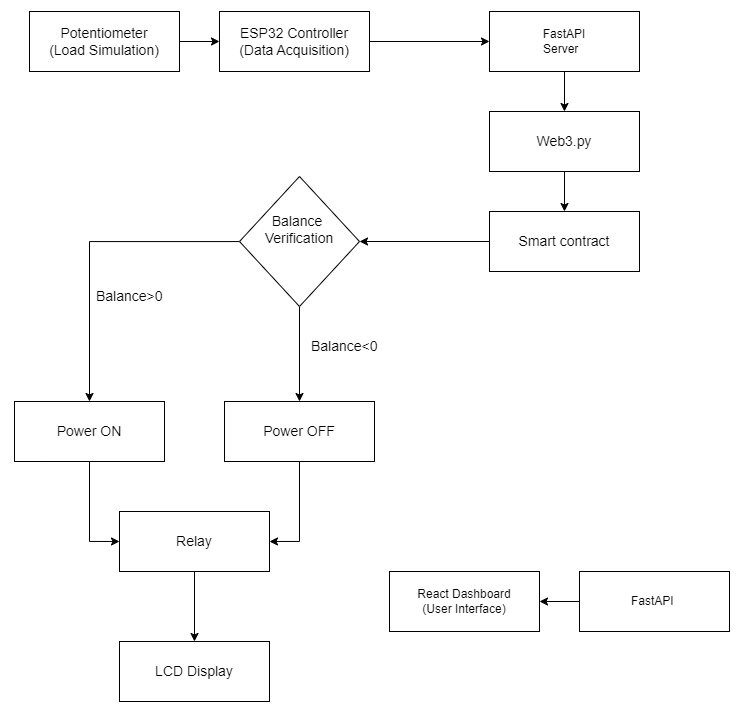
\includegraphics[width=0.8\textwidth]{Graphics/Image 1.png}
    \caption*{Figure-1: Proposed Block Diagram of decentralized power grid.\cite{ref4}}
    \label{fig:blockdiagram}

\end{figure}

\section{System Design}
The architectural framework of the system is structured across three interconnected operational layers that establish a secure, physical-to-digital automation loop.
\begin{figure}[h!]
    \centering
    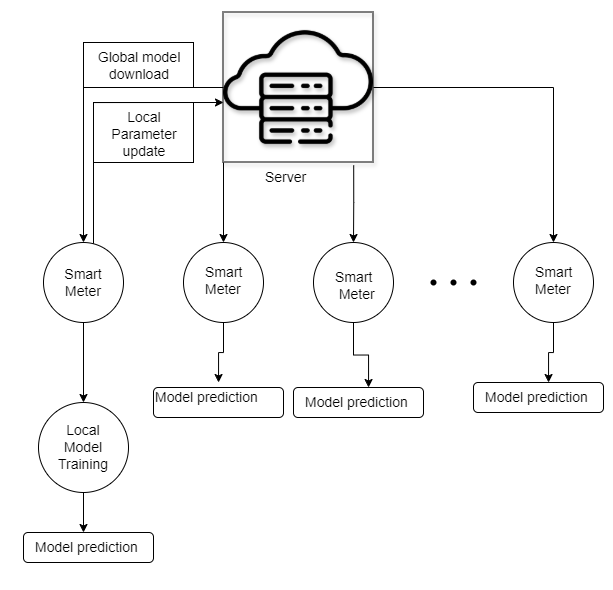
\includegraphics[width=0.8\textwidth]{Graphics/architecture.png}
    \caption*{Figure-2: System Design for decentralized power grid. \cite{ref5}}
    \label{fig:architecurediagram}
\end{figure}
\section{Tools and Techniques}
\begin{itemize}
\item Hardware: ESP32, Potentiometer, Battery

\item Software: Arduino IDE (C++), FastAPI (Python), Hardhat (Solidity), React, SQLite
\end{itemize}



\section{Data Sources}
\subsection{Primary Sources}
Real-time, low-voltage consumption data will be generated during prototype testing by the ESP32 edge node via manual potentiometer manipulation.
\subsection{Synthetic Data (Machine Learning Training)}
To properly train the predictive budgeting and anomaly detection models, a comprehensive synthetic time-series dataset will be programmatically generated using Python. This synthetic dataset will simulate thousands of regular residential consumption cycles based on time-of-day variables.

\section{Implementation}
\subsection{Hardware Layer Implementation}
The physical edge node is built around an ESP32 microcontroller configured within the Arduino IDE using C++. The firmware initializes a continuous hardware execution loop that samples analog signals from the potentiometer via the onboard Analog-to-Digital Converter (ADC) pin.
\subsection{Blockchain Ledger Implementation}
The transaction layer relies on an automated Solidity smart contract compiled, tested, and optimized within a local Hardhat. The contract design establishes state variables that map specific user cryptographic wallet addresses to their remaining token credits and device state logs (Active or Inactive). Prepaid balance tracking is processed immutably using the deduction calculation:  \cite{ref6}$$\text{Bal}_{\text{new}} = \text{Bal}_{\text{current}} - (\Delta\text{E} \times \text{R}_{\text{fees}})$$
\subsection{Backend Middleware and ML Integration}
The central logic coordination hub is built using the FastAPI framework in Python. The backend uses the Web3.py library to maintain a persistent connection to the local blockchain environment, listening continuously for emitted ledger events.\cite{ref7}

